\chapter{Análisis limitaciones actuales}

\incomment{Antes de esto se deben haber explicado las arquitecturas de 
referencia, si no hacerlo aquí.}

El proyecto \gls{wr} ofrece dos tipos de arquitectura como referencia: la 
orientada a dispositivos que actúen como \gls{bc}, y la enfocada a nodos 
finales \gls{oc}. En la sección ?? se ha visto que para la primera se cuenta 
con un dispositivo de referencia, el \gls{wrs}, que implementa la arquitectura 
de \gls{bc} y en la cual se centra el desarrollo \textit{oficial}. La segunda 
se materializa en la tarjeta \gls{spec} como ejemplo básico de nodo \gls{wr}.

La línea de desarrollo seguida desde la empresa Seven Solutions y desde el 
grupo de investigación enfocado en \gls{wr} de la UGR se ha centrado en el 
desarrollo de las arquitecturas de referencia y en el diseño de nuevos tipos de 
arquitecturas que solucionen las deficiencias presentes en los diseños 
iniciales.

Aunque la estrategía no es la misma si se habla de la arquitectura de 
\textit{switch} que si se hace de la de nodo, si es cierto que hay una 
corriente que se comparte en ambos desarrollos: la utilización de los nuevos 
modelos de \gls{soc} para lograr un mayor nivel de integración y un aumento de 
las prestaciones del sistema sin elevar la complejidad del mismo en exceso.

En el caso del \gls{wrs} existente se han detectado varios problemas por la 
gran complejidad del diseño \textit{hardware} que tiene el circuito 
electrónico. 
Uno de ellos es la comunicación entre el procesador ARM y el circuito lógico 
implementado en la lógica de la \gls{fpga}. Gracias a la mejora en la 
tecnología de fabricación se consiguen actualmente sistemas que integran tanto 
\gls{fpga} como microprocesador en un único chip reduciendo costes y 
complejidad de desarrollo.

La arquitectura referencia para los nodos \gls{wr} ha tratado de ofrecer un 
diseño básico y asequible económicamente. El uso de la familia Spartan de 
Xilinx ha permitido mantener los costes bajos a la vez que ha permitido alojar 
el diseño básico de la arquitectura de nodo \gls{wr} . Sin embargo, dicho 
diseño se está mejorando y está recibiendo cada vez más funcionalidades por lo 
que la necesidad de recursos está creciendo. Además, dicho diseño tiene una 
limitación bastante importante: carece de un microprocesador dedicado lo que 
dificulta en gran medida el desarrollo e incorporación de nuevas 
características. De igual forma que en la arquitectura de \textit{wrs} se 
tiende hacía soluciones en \gls{soc}, la arquitectura de nodo se puede 
beneficiar de este tipo de soluciones ya que permiten incluir un 
microprocesador físico en el diseño sin necesidad de gastar puertas para 
incluirlo y además mantener los costes bajos.

Mi trabajo de investigación se ha enfocado en la arquitectura de nodo por lo 
que será a la que haga referencia en el resto de la memoria, aunque como he 
comentado en los párrafos anteriores, muchas de las mejoras planteadas a 
continuación se pueden incorporar en la arquitectura tipo \textit{switch}.

\incomment{contextualizar lo siguiente}
El primer paso para poder plantear mejoras a la arquitectura de nodo y al 
rendimiento de la sincronización en los mismos es establecer el punto de 
partida. Para ello he realizado una labor de análisis de una arquitectura 
actual de nodo basada en un diseño similar al de la tarjeta \textit{spec} pero 
que ya presenta una serie de mejoras.

%\input{teoria/05_01_wrc2p_len}

El nodo utilizado como punto de partida es el WR-LEN \incomment{citar} 
desarrollado por Seven Solutions. Dicho dispositivo incorpora una versión 
mejorada del \gls{wrc} denominado \gls{wrc2p} cuya principal característica es 
la inclusión de un segundo puerto físico a la arquitectura de nodo.

\subsection{White Rabbit Core Dual Port}

\incomment{añadir refs}
El \gls{wrc2p} es una extensión de la arquitectura para nodos \gls{wr} 
denominada \acrlong{wrc} \incomment{refs} que añade una segunda interfaz física 
Ethernet a la arquitectura básica mono-puerto. En la implementación actual, la 
referencia temporal es única para ambos puertos, lo que supone que el 
dispositivo puede actuar como nodo (esclavo o maestro) y como \gls{bc}, es 
decir, esclavo de un nivel superior de la jerarquía de red y maestro de un 
nivel inferior. Además, se pretenden desarrollar técnicas que habiliten la 
redundancia (hacer un cambio de referencia si un enlace se cae). 
\incomment{mejorar la redacción de eso.}

Esta nueva arquitectura de nodo extendida permite el desarrollo de dispositivos 
\gls{bc} de coste reducido que son ideales para su uso en topologías lineales, 
donde el uso de \gls{wrs}s supone una infrautilización de los puertos 
disponibles por equipo.

\begin{figure}
	\centering
	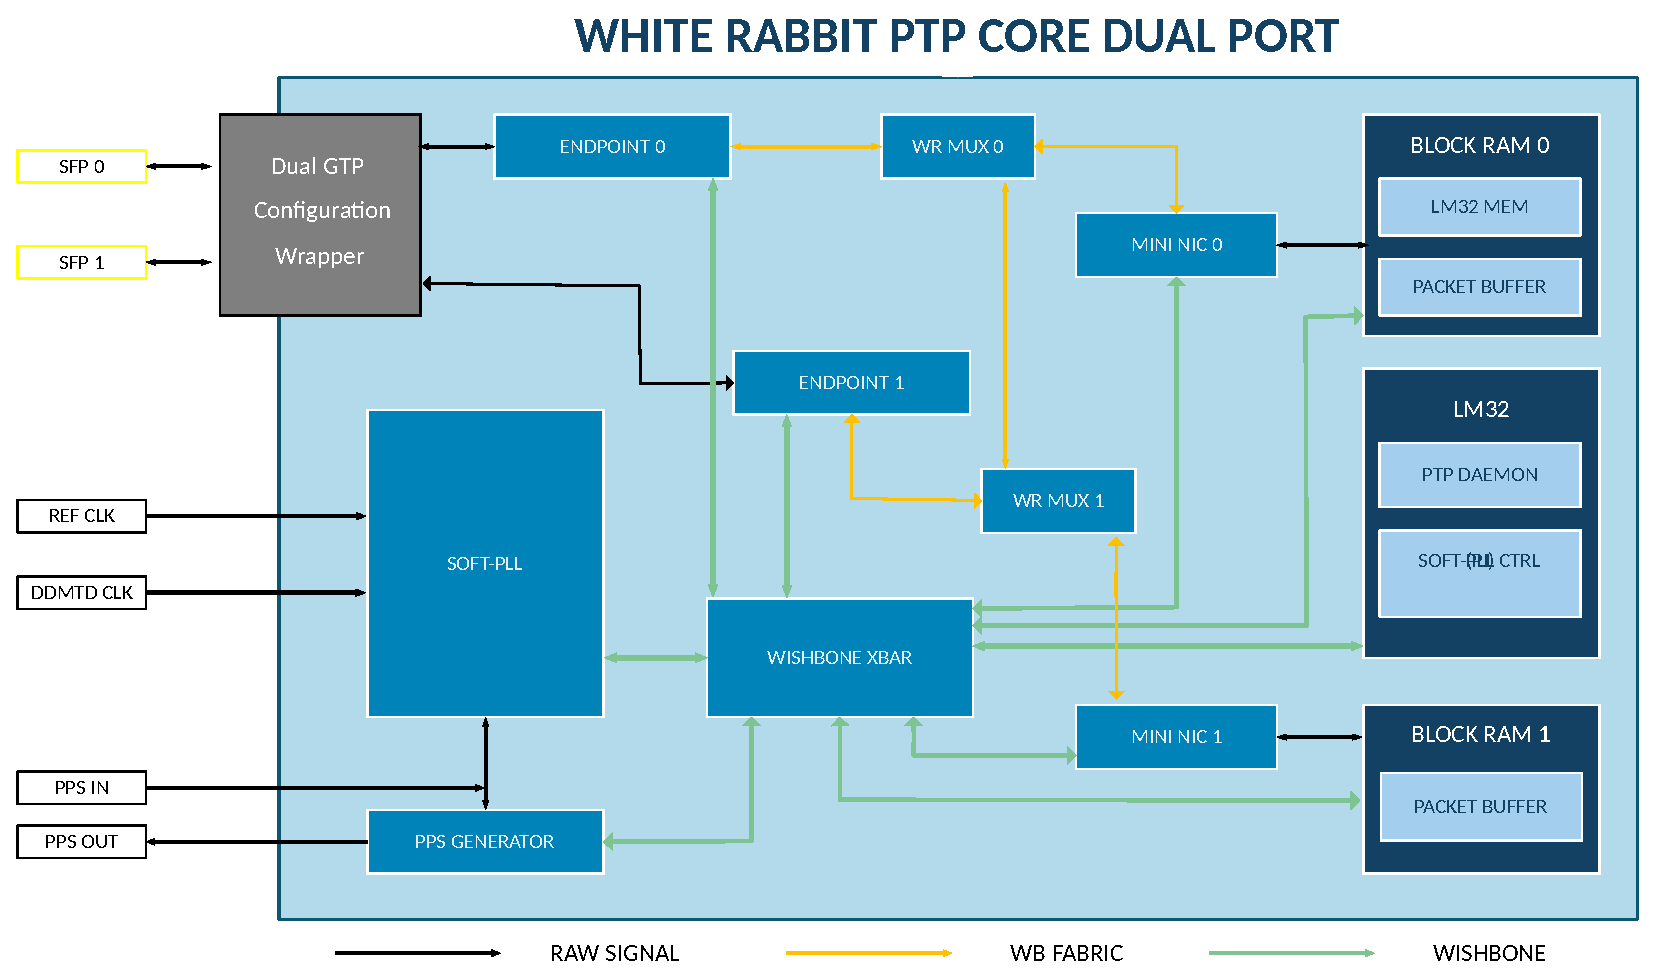
\includegraphics[width=0.7\linewidth]{imagenes/wrpc_dp}
	\caption[Diagrama de bloques del WRC2P]{Este diagrama muestra la estructura 
	de módulos HDL para el diseño de la arquitectura WRC2P.}
	\label{fig:wrpcdp}
\end{figure}


La Figura \ref{fig:wrpcdp} muestra como se organizan los módulos para la 
arquitectura de \gls{fpga}. Con respecto al diseño de referencia se realiza una 
duplicación de los componentes principales de la lógica de \gls{wr}: 
\textit{endpoint}, multiplexor WR, mini-NIC \incomment{se menciona antes nic?} 
y los módulos de RAM. Sin embargo el bloque para el procesador embebido se 
mantiene, realizando únicamente cambios a nivel de \textit{sw}. Con ello se 
consigue reducir el número de puertas necesarias, algo clave para alojar la 
arquitectura dentro de una FPGA de perfil bajo.

\subsection{WR-LEN}

El WR-LEN es el primer dispositivo \gls{wr} en incorporar la arquitectura 
\gls{wrc2p}. Fue diseñado por la empresa Seven Solutions y está disponible 
desde 2015. Sus principales características son la inclusión de un segundo 
puerto físico compatible con \gls{wr}, conectores coaxiales de tipo \gls{sma} y 
una tercera interfaz Ethernet de tipo 1000BaseT.

\begin{figure}
	\centering
	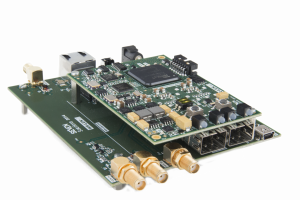
\includegraphics[width=0.7\linewidth]{imagenes/wrlen}
	\caption[WR-LEN en su versión para desarrolladores]{Imagen de un equipo 
	WR-LEN sin caja. Se puede observar como se compone de dos tarjetas: la 
	principal (arriba) donde se sitúa la electrónica de control de WR, y el 
	\textit{backplane} (abajo) que dota de interfaces de entrada/salida a la 
	primera.}
	\label{fig:wrlen}
\end{figure}


La electrónica encargada de la recuperación de reloj y mantenimiento de la 
referencia de tiempo local se mantiene con respecto a la utilizada en el 
\gls{wrs}. \incomment{si antes no se ha hablado del wrs elec. hablar aquí} El 
único cambio reseñable se encuentra en el reloj utilizado para los módulos 
\gls{ddmtd} que ya no utiliza un \gls{pll} externo para generar la frecuencia 
de 62.5 MHz necesaria, si no que se aprovecha uno de los \gls{pll} internos de 
la \gls{fpga} para ello. \incomment{que hice con los resultados?}

\subsection{Experimentos de escalabilidad}

Para evaluar las limitaciones del \gls{wrc2p} en cuanto a prestaciones y 
escalabilidad realicé una serie de experimentos encadenando múltiples nodos 
\gls{wr}. A través del análisis de la señal de reloj de salida, producida por 
la lógica de \gls{wr} se pueden obtener indicadores de como de estable es el 
proceso de sincronización en cada nodo, o dicho de otra forma, cuanto ruido 
electromagnético se añade a la señal fundamental de \gls{wr} por cada salto. 
Dichos resultados permiten establecer los límites de la implementación 
(comprobar si se cumple la exactitud sub-nanosegundo) y detectar las 
deficiencias o mejoras posibles a fin de poder mejorar el diseño existente.



\begin{figure}
	\centering
	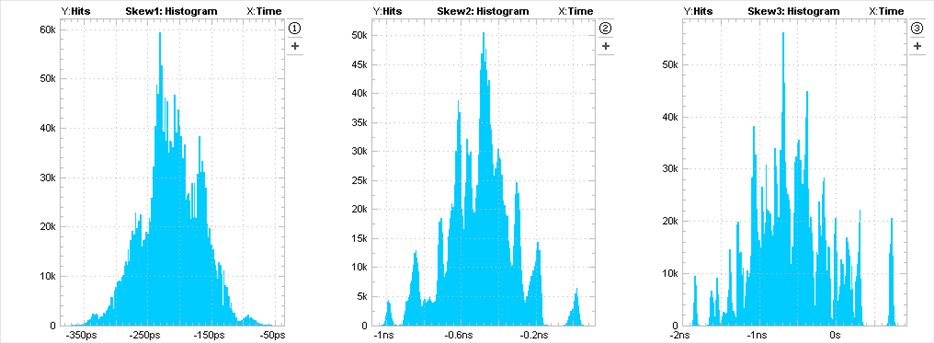
\includegraphics[width=0.7\linewidth]{imagenes/hist_exp1}
	\caption[Histograma para cadena de 18 WR-LEN]{Los histogramas muestran la 
	distribución de las muestras correspondientes a la diferencia entre las 
	señales de PPS en el maestro y la de los nodos 10, 15 y 18.}
	\label{fig:histexp1}
\end{figure}

\begin{figure}
	\centering
	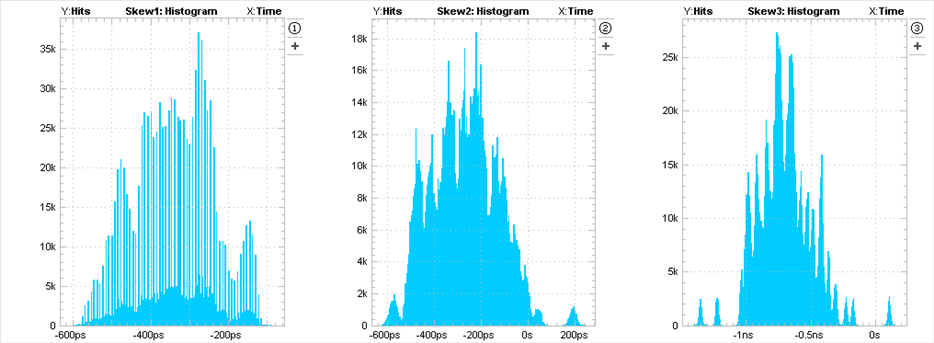
\includegraphics[width=0.7\linewidth]{imagenes/hist_exp3}
	\caption[Histograma para cadena de 18 WR-LEN]{Los histogramas muestran la 
		distribución de las muestras correspondientes a la diferencia entre las 
		señales de PPS en el maestro y la de los nodos 10, 15 y 18.}
	\label{fig:histexp2}
\end{figure}

\begin{figure}
	\centering
	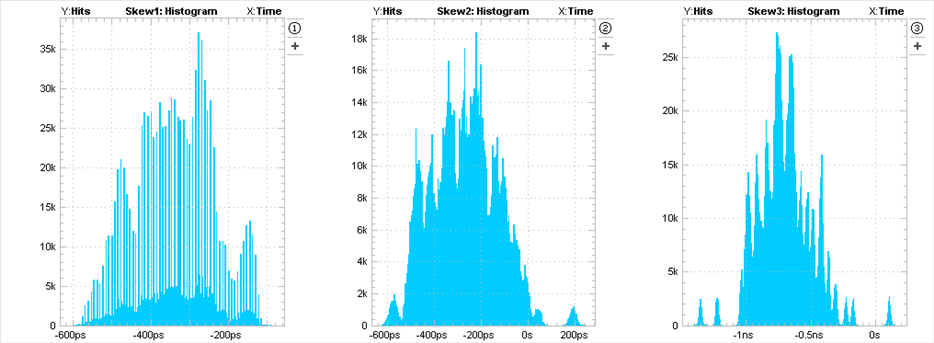
\includegraphics[width=0.7\linewidth]{imagenes/hist_exp3}
	\caption[Histograma para cadena de 18 WR-LEN]{Los histogramas muestran la 
		distribución de las muestras correspondientes a la diferencia entre las 
		señales de PPS en el maestro y la de los nodos 10, 15 y 18.}
	\label{fig:histexp3}
\end{figure}


